\documentclass[12pt]{article}
%preamble for latex
\usepackage{amsmath,listings}
\usepackage{graphicx,color}
\usepackage[margin=1.3in]{geometry}
\usepackage[english]{babel}
\usepackage[utf8]{inputenc}
\usepackage[colorinlistoftodos]{todonotes}
\usepackage{url}
\usepackage{listings}
\usepackage{hyperref}
\hypersetup{
    colorlinks=true,
    linkcolor=blue,
    filecolor=magenta,      
    urlcolor=blue,
}
\usepackage{color}
\usepackage{textcomp} 
 
\usepackage[nottoc]{tocbibind}

\definecolor{codegreen}{rgb}{0,0.6,0}
\definecolor{codegray}{rgb}{0.5,0.5,0.5}
\definecolor{codepurple}{rgb}{0.58,0,0.82}
\definecolor{backcolour}{rgb}{0.95,0.95,0.92}
  
\lstdefinestyle{mystyle}{
    backgroundcolor=\color{backcolour},   
    commentstyle=\color{codegreen},
    keywordstyle=\color{magenta},
    numberstyle=\tiny\color{codegray},
    stringstyle=\color{codepurple},
    basicstyle=\footnotesize,
    breakatwhitespace=false,         
    breaklines=true,                 
    captionpos=b,                    
    keepspaces=true,                 
    numbers=left,                    
    numbersep=5pt,                  
    showspaces=false,                
    showstringspaces=false,
    showtabs=false,                  
    tabsize=2
}
 
\lstset{style=mystyle}

\begin{document}
\begin{titlepage}

\center % Center of the page
 
%----------------------------------------------------------------------------------------
%	Assignment Number
%----------------------------------------------------------------------------------------


{ \Large \textbf {Assignment 8}}\\[1.0cm] % Title of your document

%----------------------------------------------------------------------------------------
%	HEADING
%----------------------------------------------------------------------------------------

\textsc{\LARGE \textbf{ELP 780 Software Lab}\\[1.0cm]} % Course Code 
\textsc{\Large \textbf{Varun Sood}  }\\[.5cm] % Author's Name 
\textsc{\Large \textbf{2017EET2839}  }\\[0.5cm] % ROll
\textsc{\Large \textbf{2017-19}  }\\[1.5cm] % Year of entry
\textmd{\large {A report for the assignment on}  }\\[0.5cm] % Year of entry
\textsc{\large Python Programs }\\[3cm] % Year of entry


%----------------------------------------------------------------------------------------
%	LOGO 
%----------------------------------------------------------------------------------------


\includegraphics[scale=.5]{logo.png}\\[1cm] 

\Large\textbf{{Bharti School of}}\\
\Large\textbf{{Telecommunication Technology and Management}}\\
\Large\textbf{{IIT DELHI}}\\
\Large\textbf{{India}}\\



%----------------------------------------------------------------------------------------
%	DATE SECTION
%----------------------------------------------------------------------------------------

{\large \today}\\[3cm] % Date

\end{titlepage}
  
%Creating a table of content for the report
\pagebreak
\tableofcontents
\pagebreak

\pagenumbering{arabic}
\section{Problem Statement 1}
\subsection{Problem statement}{
\textbf{}
Find the two largest valid crosses that can be drawn on smart cells in the grid, and return two integers denoting the dimension of the each of the two largest valid crosses. In the above diagrams, our largest crosses have dimension of 1,  5 and 9 respectively .\\

\textbf{Note:} The two crosses cannot overlap, and the dimensions of each of the valid crosses should be maximal.\\


\subsection{Assumptions}
{
\begin{itemize}
\item The input file name is taken from the user.
\item The file format is given by the user.
\item Program is assumed to be run only once and files deleted which were created before running again.

\end{itemize}
}

\subsection{Program Structure}

{
\begin{center}
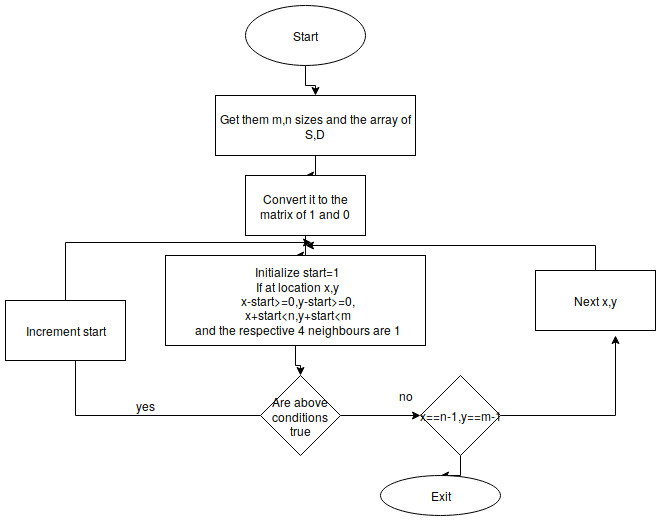
\includegraphics[width=0.8\textwidth]{ps1.jpg}\\
\end{center}
}
\newpage

\subsection{Algorithm and Implementation}
{\begin{itemize}
\item First get the elements and 2 d array.
\item Generate a matrix of 1 and 0, 1 for the S and 0 for the D.
\item Loop over the matrix trying to increase the dimension of the cross in each dimension.
\item If true for 1 value of start increase start test again in all 4 directions, up, down , left and right.
\end{itemize}
}
\subsection{Input and Output Format}
{
\begin{itemize}

\item \textbf{Input format} \\
The first line contains two space-separated integers,  n and m.\\
Each of the next  lines n contains a string of  m characters where each character is either S (Smart) or D (Dull). These strings represent the rows of the grid. If the jth character in the ith  line is S, then  (i,j) is a  cell smart. Otherwise it's a  dull cell.

\item \textbf{Output format} \\
Print 2 maximums bigger first.\\
\end{itemize}
}
\subsection{Test Cases}
{\textbf{Input} \\
5 6\\
SSSSSS\\
SDDDSD\\
SSSSSS\\
SSDDSD\\
SSSSSS\\
\textbf{Output}\\
5 1\\
}
\subsection{Difficulty/Issues faced}
{
\begin{itemize}
\item Python donot define data type at initialization so error might crop up.
\item latex is difficult to use
\item Python is different then the previous languages..
\end{itemize}
}
\subsection{Screenshots}
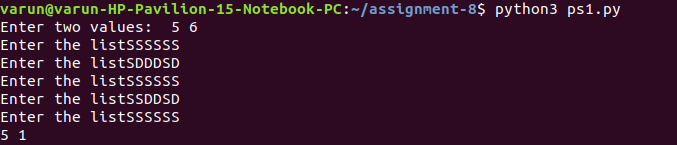
\includegraphics[width=0.8\textwidth]{out1.png}
\begin{center}
\textbf{Final output}
\end{center}

\pagebreak
\section{Problem Statement 2}
{\textbf{}
After, getting mix results of valid crosses, professors decided to test the computation abilities on one more problem. This time professors wanted to test the decryption capabilities of the computer.
Encryption of  a message requires three keys, k1, k2, and k3. The 26 letters of English and underscore are divided in three groups,  [a-i] form one group, [j-r] a second group, and everything else ([s-z] and underscore) the third group. Within each group the letters are rotated left by ki positions in the message. Each group is rotated independently of the other two. Decrypting the message means doing a right rotation by ki positions within each group.

}

\subsection{Assumptions}
{
\begin{itemize}
\item The input file name is taken from the user.
\item The file format is given by the user.
\item Program is assumed to be run only once and files deleted which were created before running again.
\end{itemize}
}
\subsection{Program Structure}
\begin{center}
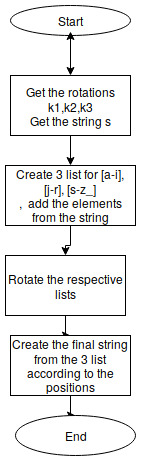
\includegraphics[width=0.2\textwidth]{ps2.jpg}\\
\end{center}

\subsection{Algorithm and Implementation}
{\begin{itemize}
\item Input values of rotation k1,k2,k3 are taken from the user.
\item Input string is taken from the user.
\item Get the different strings out in  3 different lists.\\
\item Rotate them and atlast add them in the string.
\item Print the string.
\end{itemize}
}
\subsection{Input and Output Format}
{
\begin{itemize}

\item \textbf{Input format} \\
k1 k2 k3\\
string\_sample\\

\item \textbf{Output format} \\
rotated\_string\\
\end{itemize}
}


\subsection{Test Cases}
{
\textbf{Input}\\
2 3 4\\
dikhtkor\_ey\_tec\_ocsussys.exit()rsw\_ehas\_\\
\textbf{Output}\\
hardwork\_is\_the\_key\_to\_success\\

}
\subsection{Difficulty/Issues faced}
{
\begin{itemize}
\item Python donot define data type at initialization so error might crop up.
\item latex is difficult to use
\item Python is different then the previous languages..
\end{itemize}
}
\subsection{Screenshots}
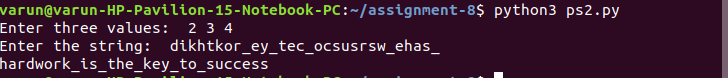
\includegraphics[width=0.8\textwidth]{out2.png}
{
\begin{center}
    
\end{center}    
}
\newpage

\section{Appendix}

\subsection{Appendix-A : code for ps1}
\textbf{code1}
\begin{lstlisting}[language=python,caption=ps1.py]
{
###### this is the first .py file ###########
#!/usr/bin/python
import sys
import copy
####### write your code here ##########
inp = input("Enter two values:  ").split(" ")
#inp = raw_input("Enter two values:  ").split()
#give input to the 
n = int(inp[0])
m = int(inp[1])
if n<=1 or n >=106:
    print("Enter proper variable")
    sys.exit()
if m<=1 or m >=106:
    print("Enter proper variable")
    sys.exit()
#a list
a=[]
str1=[]
#get the list 
for i in range(n):
    #l = input("Enter the list")
    l = input("Enter the list")
    for j in range(len(l)):
        str1.append(l[j])
        str2=copy.copy(str1)
    a+=[str2]
    del str1[0:len(str1)]
#print(a)
#new matrix
Matrix1 = [[0 for x in range(m)] for y in range(n)] 
for x in range(n):
    for y in range(m):        
        if(a[x][y]=='S'):
           Matrix1[x][y] = 1
        else:
           Matrix1[x][y] = 0
#max2 and max1 are maximums top 2
max2=0
max1=0
mat=[]
valid=1
# to find out the cross in the matrix
for x in range(n):
    for y in range(m):        
        if(Matrix1[x][y]==1):
            start=0
            valid=1
            #while valid increase valid
            while (valid==1):
                if(x>=start):
                    if(Matrix1[x-start][y]==1):
                        pass
                    else:
                        valid=0    
                        break
                else:
                    valid=0         
                    break
                
                if(y>=start):
                    if(Matrix1[x][y-start]==1):
                        pass
                    else:
                        valid=0
                        break
                else:
                    valid=0
                    break

                if(x+start<n):
                    if(Matrix1[x+start][y]==1):
                        pass
                    else:
                        valid=0             
                        break
                else:
                    valid=0  
                    break
                if(y+start<m):
                    if(Matrix1[x][y+start]==1):
                        pass
                    else:
                        valid=0
                        break
                else:
                    valid=0
                    break
                start=start+1
            if(max2<max1 and max1<start):
                max2=max1
            if(max1<start):
                max1=start
            mat+=[start]
            #print(start,x,y)
print(4*(max1-1)+1,4*(max2-1)+1)

}
\end{lstlisting}
\newpage

\subsection{Appendix-B : code for ps2}
\textbf{code2}
\begin{lstlisting}[language=python,caption=ps2.py]
###### this is the second .py file ###########
import sys
#rotate function
#input : list an l and length n
#output : rotate the list by  n and return the output list
def rotate(l, n):
    return l[n:] + l[:n]


#!/usr/bin/python
####### write your code here ##########
#get input
inp = input("Enter three values:  ").split(" ")
#divide it into 3 parts
k1 = int(inp[0])
k2 = int(inp[1])
k3 = int(inp[2])
if k1<1 or k1 >151:
    print("Enter proper variable")
    sys.exit()
if k2<1 or k2 >151:
    print("Enter proper variable")
    sys.exit()
if k2<1 or k2 >151:
    print("Enter proper variable")
    sys.exit()

# different parts regular expressions for matching
part1=[]
part1+='abcdefghi'        #one of the alphabets
part2=[]
part2+='jlkmnopqr'        #one of the alphabets
part3=[]
part3+='stuvwxyz_'       #one of the alphabets
#for 3 parts of the string accordint to 3 regular exp
str1=[]
str2=[]
str3=[]
#input string
string = input("Enter the string:  ")
if len(string)<1 or len(string) >151:
    print("Enter proper variable")
    sys.exit()

#convert to string
string=list(string)
#divide the string into 3 parts
for i in range(len(string)):
    if string[i] in part1:
        str1+=string[i]
        pass
    if string[i] in part2:
        str2+=string[i]
        pass
    if string[i] in part3:
        str3+=string[i]
        pass
#print(str1)
rotate(str1, k1)
#print(str2)
rotate(str2, k2)
#print(str3)
rotate(str3, k3)
#rotating the entire string according to developed lists
l=0
m=0
n=0
for i in range(len(string)):
    if string[i] in part1:
        #print(part1.index(string[i]))
        string[i]=str1[(l-k1)%len(str1)]
        l+=1
        pass
    if string[i] in part2:
        string[i]=str2[(m-k2)%len(str2)]
        m+=1
        pass
    if string[i] in part3:
        string[i]=str3[(n-k3)%len(str3)]
        n+=1
        pass
final_output = ''.join(string)
#print the final output
print(final_output)

    
\end{lstlisting}  
\newpage



\begin{thebibliography}{9}


\bibitem{Python} 
Python tutorial,\\
\url{https://www.tutorialspoint.com/python/}

\bibitem{Git} 
Tutorial point for Git,\\
\url{https://www.tutorialspoint.com/git/}

\bibitem{latex_website} 
Latex format guide,\\
\url{ https://www.sharelatex.com/}

\end{thebibliography}


\end{document}